\chapter{Results}

This chapter shows the results from running the research on the dataset. These results focus on 
correlation coefficients and the differences between artistic and statistic exemplars.

\section{Correlation Coefficient Results}
One parameter for our classifier is the choice of $k$ for $k$-Nearest Neighbour. Simply setting 
$k=1$ has the effect of assigning the year of the nearest painting in feature space to the current
test painting. Whilst setting $k=102$ has the effect of giving the painting the mean year of the 
entire data set. Obviously, a point between the two is likely to be the best. 

\begin{figure}[h]
\centering
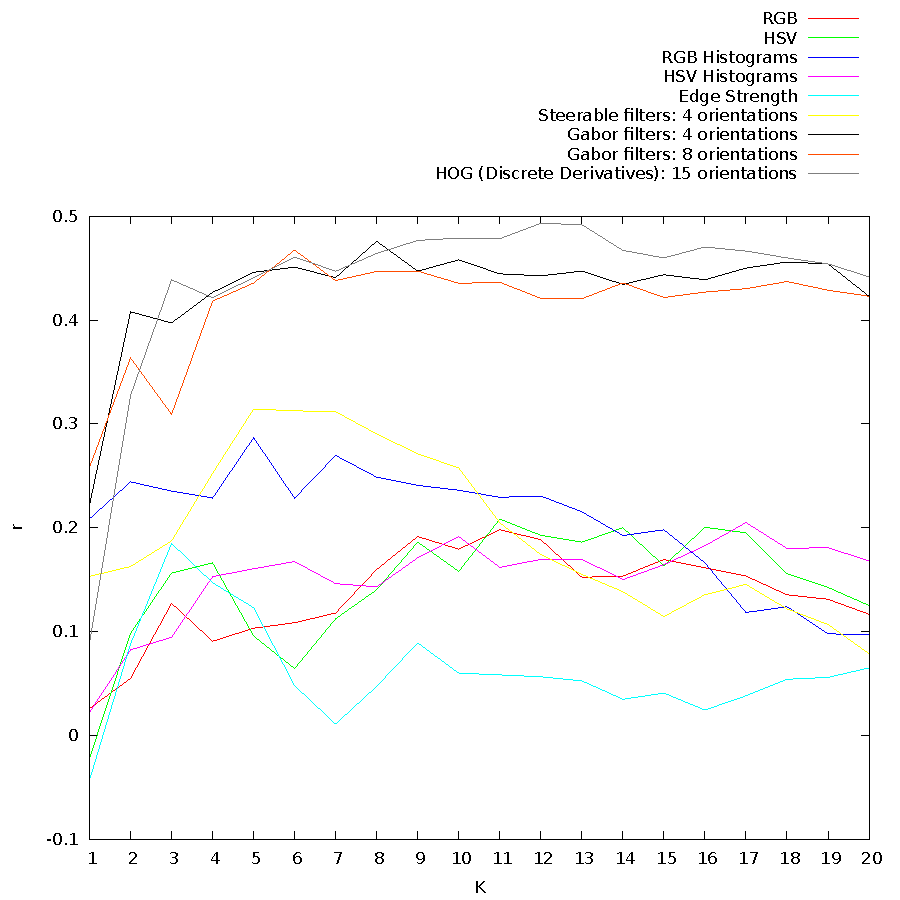
\includegraphics[width=0.9\textwidth]{../../isispa-paper/results/mean}
\caption{Correlation Coefficients $r$ against $k$ values for $k$-Nearest Neighbour}\label{fig:r-graph}
\end{figure}

From Figure~\ref{fig:r-graph} it is apparent that for many of the feature spaces we have an
optimum value of $k$ of around 7 or 8. Table~\ref{tab:r-results} shows the actual results for each 
feature space for a $k$ of 7, where $r$ is the correlation coefficient given by Pearson's, 
$P(r)$ is the p-value significance of $r$.

$C(n)$ is the percentage of paintings correctly classified within $n$ years of the actual year 
(where $E(X)-n \le X \le E(X)+n$).

\begin{table}[h]
\centering
\begin{tabular}{|l|c|c|c|}\hline
Technique     					& $r$    & $P(r)$ & $C(15)$ \\ \hline
Edge Strength 					& 0.0107 & 0.910  & 60\%    \\
HSV 						& 0.112	 & 0.237  & 64\%    \\
RGB 						& 0.118  & 0.214  & 63\%    \\
HSV Histograms					& 0.146	 & 0.123  & 64\%    \\
RGB Histograms					& 0.270	 & 0.004  & 62\%    \\
HOG (Discrete Derivatives): 4 orientations 	& 0.307	 & 0.001  & 65\%    \\
Steerable filters: 4 orientations 		& 0.312	 & 0.001  & 68\%    \\
HOG (Discrete Derivatives): 8 orientations 	& 0.346	 & \textless0.001 & 65\% \\
HOG (Discrete Derivatives): 16 orientations 	& 0.367	 & \textless0.001 & 64\% \\
Gabor filters: 16 orientations			& 0.370  & \textless0.001 & 67\% \\
Gabor filters: 8 orientations			& 0.438	 & \textless0.001 & 70\% \\
Gabor filters: 4 orientations			& 0.441	 & \textless0.001 & 71\% \\
\hline
\end{tabular}
\caption{Correlation Coefficients, ordered by strength for $k=7$}\label{tab:r-results}
\end{table}


\newpage
\section{Ensemble Results}
Using ensemble methods can both improve and weaken the correlation coefficients depending on the
techniques used. The inclusion of colour histogram analysis and HSV colour-space statistical
analysis typically weakens the results. Whilst combining \gls{hog} and Gabor filters typically 
improves the correlation coefficients beyond each technique individually. 
Table~\ref{tab:ensemble-results} shows some examples of this.

This does show that ensemble methods can help to improve the strength of analysis techniques, as
expected.

\begin{table}[h]
\centering
\begin{tabular}{|l|c|c|}\hline
Method	& $r$	& $P(r)$ \\ \hline
RGB 						& 0.118  & 0.214 \\
Ensemble RGB Histogram and HOG (16)		& 0.256 & 0.006 \\
RGB Histograms					& 0.269 & 0.004 \\
HOG (Discrete Derivatives): 16 orientations	& 0.367 & \textless0.001 \\
Ensemble RGB and HOG (16)			& 0.372 & \textless0.001 \\
Gabor filters: 4 orientations			& 0.441 & \textless0.001 \\
Ensemble RGB and Gabor (4)			& 0.443	& \textless0.001 \\
Ensemble RGB, Gabor (4) and HOG (16)		& 0.464	& \textless0.001 \\
\hline
\end{tabular}
\caption[Correlation Coefficients comparing individual and ensemble methods]{Correlation Coefficients comparing individual and ensemble methods. Note how the 
combination of RGB Histograms and \gls{hog} has decreased performance, whilst the combination of
\gls{hog} and Gabor filters has improved performance.}\label{tab:ensemble-results}
\end{table}

\newpage
\section{Exemplar Results}
The intuition -- that using artistically chosen exemplars could help to exploit knowledge about 
the way the paintings change over time -- turned out to be incorrect. Results for Gabor filters 
with 4 orientations (the best performing method in the previous experiment) are shown in 
Table~\ref{artistic_exemplars}.  Results for the other feature spaces show a similar pattern, the 
same distance measure ($\chi^2$) has been used throughout. 

\begin{table}[h]
\centering
\begin{tabular}{|p{3.5cm}|c|c|c|}
\hline
Technique     & $r$ & $P(r)$ & $C(15)$ \\ \hline
%K=7
Artistic Exemplars	& 0.328	& \textless0.001 & 57\%\\
Statistical Exemplars	& 0.383	& \textless0.001 & 61\%\\
Centroid		& 0.403	& \textless0.001 & 64\%\\
\hline
\end{tabular}
\vspace{0.5em}
\caption{Correlation coefficients, ordered by strength, for Exemplars
\label{artistic_exemplars}}
\end{table}

These exemplars give an interesting insight into the feature space. The paintings shown in 
Figures~\ref{early_example} and~\ref{late_example} are both artistic exemplars, however the 
earlier painting ``\emph{Snowdon, the Traeth and the Frightened Horse}'', from 1948, is far from 
the feature space centroid for that year, whereas the later painting is very close to the feature 
space centroid for 1985. A visualisation of artistic exemplars and their corresponding statistical
representations is given in Figure~\ref{art_ex_stat_ex}. From this you can see that artistic 
information does not necessarily correspond well to the feature space(s) we use. Note that whilst 
Figure~\ref{art_ex_stat_ex} uses the feature space defined by Gabor filters with 4 orientations, 
our best performing: the pattern is similar for all other feature spaces.

\begin{figure}[h]
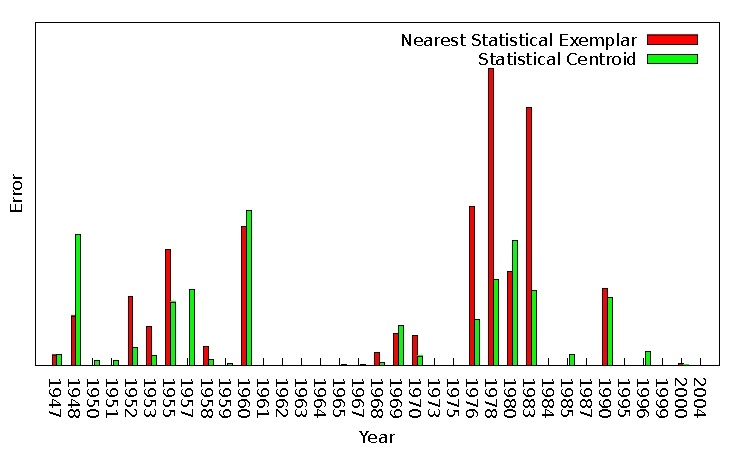
\includegraphics[width=\linewidth]{img/exemplar.pdf}
\caption[Distance in feature space from artistic to statistic exemplars]{Distance in feature space from artistic to statistic exemplars (red); distance from 
artistic exemplar to centroid (green). Lower values indicate that the artistic exemplar is near to
the mean painting for a particular year, higher values that an artistic exemplar painting is an 
outlier for this particular feature space\label{art_ex_stat_ex}}
\end{figure}
